\item \textbf{Summarize your findings and observations briefly in a final discussion. Submit both the developed code and your document to the Assignment 3 folder on D2L.}
\begin{enumerate}
\item Although re-sampling has some positive effects on features extracting part (deleting zeros padding parts), it could decrease the quality of spectral features. For example, the algorithm could not find any features for this part of the signal because the scale of STFT was changed (see figure \ref{fig:Ass3_Q2_Peak_freq}). Therefore, we need to update our algorithm for finding peaks or extract other features.

\begin{figure}[H]
    \centering
    \begin{minipage}[b]{1\textwidth}
        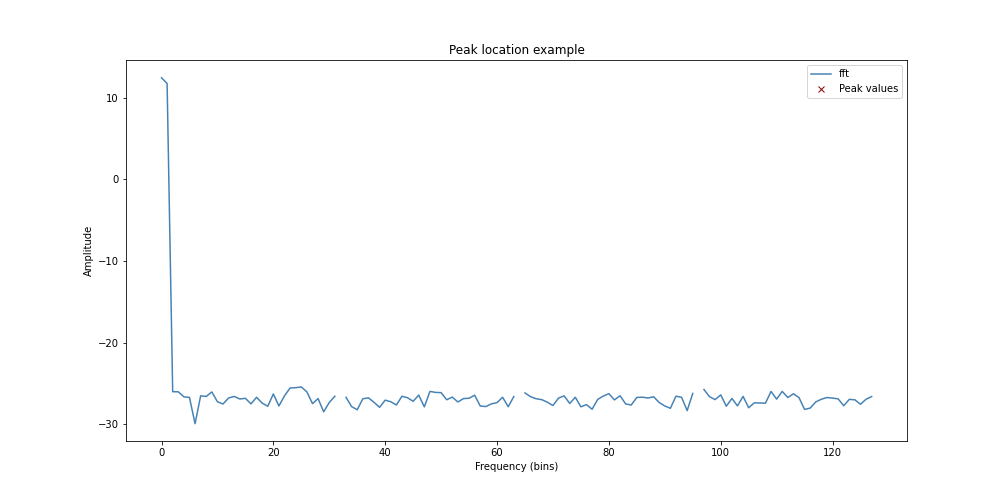
\includegraphics[width=\textwidth]{manuscript/src/figures/Ass3/Ass3_Q2_Peak_freq.png}
    \end{minipage}
    \caption{The magnitude of STFT and its peak values.}
    \label{fig:Ass3_Q2_Peak_freq}
\end{figure}

\item Data normalization had a significant effect on the result of HMM (compare figures \ref{fig:Ass3_Q2_states_user_3} and \ref{fig:Ass3_Q2_states_user_10} with \ref{fig:Ass3_Q2_states_user_3N} and \ref{fig:Ass3_Q2_states_user_10N}, respectively)

\item The decoding result was not good enough for finding different states in raw data. The reason for this result could be either the re-sampling of data or the size of the training set.


\end{enumerate}
